\documentclass[../main.tex]{subfiles}

\begin{document}

\section{Parity violation}%
\label{sec:parity_violation}

We weten uit experimenten dat de zwakke interactie gegeven wordt door de groep $SU(2)$.

\subsection{Pariteit}%
\label{sub:pariteit_rev}

Kijken we eerst terug naar de definitie die we aan pariteit hebben gegeven in sectie \ref{sub:pariteit}. Dit is niets anders dan het systeem spiegelen door de oorsprong. Voor vectoren krijgen we dan
\begin{equation}
    \begin{aligned}
        \label{eq:pariteit_rev}
        P(\vec{r}) &= -\vec{r}\\
        P(\vec{p}) &= -\vec{p}\\
    \end{aligned}
\end{equation}
en voor axiale vectoren
\begin{equation}
    \begin{aligned}
        \label{eq:pariteit_ax}
        \vec{L} &= \vec{r} \times \vec{p}\\
        p(\vec{L}) &= \vec{L}
    \end{aligned}
\end{equation}
De eigenwaardes van de toestanden die de pariteit volgen zijn $\pm 1$.

\subsubsection{Dirac fermionen}%
\label{ssub:dirac_fermionen}

Uit de dirac vergelijking was het mogelijk om 4 onafhankelijke oplossingen waren
\begin{equation}
    \begin{aligned}
        \label{eq:dirac_fermions}
        \begin{matrix}
            u_1 = \sqrt{E+m}
            \begin{pmatrix}
                1\\
                0\\
                \frac{p_z}{E+m}\\
                \frac{p_x + ip_y}{E+m} 
            \end{pmatrix} &
            u_2 = \sqrt{E+m}
            \begin{pmatrix}
                0\\
                1\\
                \frac{p_x - ip_y}{E+m} 
                \frac{-p_z}{E+m}\\
            \end{pmatrix} \\
            v_2 = \sqrt{E+m}
            \begin{pmatrix}
                \frac{p_z}{E+m}\\
                \frac{p_x + ip_y}{E+m}\\ 
                1\\
                0
            \end{pmatrix} &
            v_1 = \sqrt{E+m}
            \begin{pmatrix}
                \frac{p_x - ip_y}{E+m} \\
                \frac{-p_z}{E+m}\\
                0\\
                1
            \end{pmatrix}
        \end{matrix}
    \end{aligned}
\end{equation}
Hierbij stellen de $u$'s deeltjes voor en de $v$'s de antideeltjes. waarbij we hebben dat $v_1(E,\vec{p})e^{-i(\vec{p}\cdot \vec{x}-Et)} = u_4(-E,-\vec{p})e^{-i(-\vec{p}\cdot -\vec{x}-(-E)t)}$. $v_1$ is dus niets anders dan een deeltje dat terug gaat in de tijd met negatieve energie en impuls. Voeren we nu de pariteits operator uit op de dirac vergelijking dan krijgen we:
\begin{equation}
    \begin{aligned}
        \label{eq:dirac_par}
        i\gamma^1 \frac{\partial \psi}{\partial x} + \dotsc -m\psi &= -i\gamma^0 \frac{\partial \psi}{\partial t} \\
                                                                   &\downarrow \psi \rightarrow \hat{P}\psi\\
        i\gamma^1 \hat{P} \frac{\partial \psi'}{\partial x} + \dotsc -m \hat{P} \psi' &= -i\gamma^0 \hat{P} \frac{\partial \psi'}{\partial t} \\
                                                                                      &\downarrow t\rightarrow t, x\rightarrow -x \Rightarrow \gamma^0\\
        -i\gamma^0\gamma^1 \hat{P} \frac{\partial \psi'}{\partial x'} + \dotsc -m \gamma^0 \hat{P} \psi' &= -i\gamma^0\gamma^0 \hat{P} \frac{\partial \psi'}{\partial t'} \\
                                                                                                         &\downarrow \gamma^0\gamma^k = -\gamma^k\gamma^0\\
        i\gamma^1\gamma^0 \hat{P} \frac{\partial \psi'}{\partial x'} + \dotsc -m \gamma^0 \hat{P} \psi' &= -i\gamma^0\gamma^0 \hat{P} \frac{\partial \psi'}{\partial t'} \\
                                                                                                       &\Updownarrow\\
        i\gamma^1 \frac{\partial \psi'}{\partial x'} + \dotsc -m\psi' &= -i\gamma^0 \frac{\partial \psi'}{\partial t'} 
    \end{aligned}
\end{equation}
Uit de onderste 2 vergelijkingen die gelijk zijn aan elkaar zien we dat $\gamma^0 \hat{P}$ niet anders is dan de eenheidsoperator. Hieruit is $\hat{P}=+\gamma^0$ of $\hat{P}=-\gamma^0$. Bij conventie hebben we genomen dat $\hat{P}=+\gamma^0$ en krijgen we voor de inwerking van de pariteit op de dirac oplossingen:
\begin{equation}
    \begin{aligned}
        \label{eq:par_dirac_opl}
        \begin{matrix}
            \gamma^0u_1 = +u_1 & \gamma_0u_2 = +u_2 \\
            \gamma^0v_1 = -v_1 & \gamma_0v_2 = -v_2 \\
        \end{matrix}
    \end{aligned}
\end{equation}
De positieve deeltjes hebben dus een positieve pariteit en de negatieve deeltjes een negatieve pariteit.

\subsubsection{QED}%
\label{ssub:qed}

Dit heeft natuurlijk gevolgen voor de wiskunde die we al eerder hebben aangehaald. Kijken we eerst wat dit zal doen bij QED. Als voorbeeld bekijken we een elektron muon verstrooiing $e^-\mu\rightarrow e^-\mu$. Het matrix element hiervan is 
\begin{equation}
    \begin{aligned}
        \label{eq:e_mu_pariteit}
        \mathcal{M}= \frac{e^2}{q^2} j_e\cdot j_\mu
    \end{aligned}
\end{equation}
met $j_e^\mu = \overline u(p_3)\gamma^\mu u(p_1)$ en $j_\mu^\nu = \overline u(p_4)\gamma^\nu u(p_2)$.

\begin{figure}[h]
    \centering
    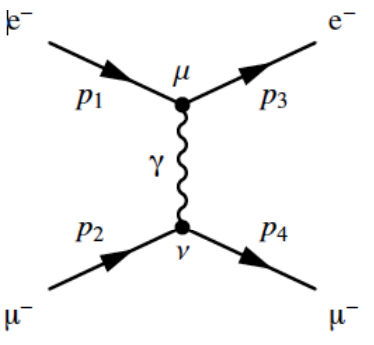
\includegraphics[width=0.4\linewidth]{parity_violation/diagram_e_mu.png}
    \caption{Feynman diagram van $e^- \mu$ botsing}%
    \label{fig:parity_violation/diagram_e_mu}
\end{figure}

Het transformeren van het matrix element gaat nu als volgt:
\begin{equation}
    \begin{aligned}
        \label{eq:qed_mat_par}
        u &\rightarrow \gamma^0 u\\
        \overline u = u^\dagger \gamma^0 &\rightarrow (\gamma^0u)^\dagger \gamma^0=u^\dagger\gamma^0\gamma^0 = \overline u \gamma^0\\
                                         &\Downarrow\\
        j_e^\mu = \overline u(p_3)\gamma^\mu u(p_1) &\rightarrow \overline u(p_3)\gamma^0\gamma^\mu\gamma^0 u(p_1)
    \end{aligned}
\end{equation}
Bekijken we de tijd en ruimte componenten apart:
\begin{itemize}
    \item Tijd component:
        \begin{equation}
            \begin{aligned}
                \label{eq:qed_mat_par_tijd}
                j_e^0 \rightarrow \overline u\gamma^0\gamma^0\gamma^0 u &= \overline u \gamma^0 u = j_e^0\\
                \gamma^0\gamma^0&=I
            \end{aligned}
        \end{equation}
    \item Ruimte component:
        \begin{equation}
            \begin{aligned}
                \label{eq:qed_mat_par_ruimte}
                j_e^k \rightarrow \overline u\gamma^0\gamma^k\gamma^0 u &= \overline u\gamma^k\gamma^0\gamma^0 u = -j_e^k\\
                \gamma^k\gamma^0&=-\gamma^0\gamma^k
            \end{aligned}
        \end{equation}
\end{itemize}
Zo krijgen we uiteindelijk voor het scalair product van de stromen dat
\begin{equation}
    \begin{aligned}
        \label{eq:qed_stromen_par}
        j_e\cdot j_\mu = j_e^0j_\mu^0 - j_e^kj_\mu^k \rightarrow j_e^0j_\mu^0 - (-j_e^k)(-j_\mu^k) = j_e\cdot j_\mu
    \end{aligned}
\end{equation}
Met andere woorden QED behoud de pariteit. Omdat QCD juist dezelfde stromen hebben met enkel andere voorfactoren en propagatoren kunnen we zeggen dat QCD pariteit ook zal behouden.

\subsection{Pariteit schenden in experimenten}%
\label{sub:pariteit_schenden_in_experimenten}

Als we terug kijken in de geschiedenis ontstaat er ehet $\theta/\tau$ probleem. Hierbij werden er bij $\pm500$MeV 2 mesonen onntdekt die ongeveer dezelfde massa hebben maar ze zien aan de hand van hun vervalmodes dat het andere deeltjes zijn, $\theta^+\rightarrow 2\pi$ en $\tau^+\rightarrow 3\pi$. We verwachten dat $\theta$ veel sneller zou vervallen dan $\tau$ en dus een veel breedere piek zou hebben. Uit meer precieze metingen bleek dat dit één en hetzelfde deeltje waren met juist dezelfde massa en levensduur. Dit zorgt natuurlijk voor problemen. De 2 deeltjes hebben een tegengestelde pariteit en zouden volgens het behoud van pariteit onmogelijk hetzelfde deeltje kunnen zijn. Lee en Yang komen met het voorstel dat de pariteit niet behouden zou zijn bij zwakke vervallen en dat $\theta^+ = \tau^+ \equiv K^+$. Zij vragen aan C.S. Wu om dit experimenteel na te gaan. Zij heeft dit gedaan door het onderzoek van $\beta$-verval van gepolariseerde $^{60}$Co waaruit volgt dat de pariteit niet behouden is. Waaruit de V-A theorie zal volgen

\subsection{Wu-experiment}%
\label{sub:wu_experiment}

De cross sectie is niets meer dan een waarschijnlijkheid/getal. Dit kan ofwel een scalair of een pseudoscalair zijn. Indien de cross sectie niet van teken verrandert is het een scalair en is $P$ behouden. Indien de cross sectie wel van teken verrandert is het een pseudoscalair en zal de P niet behouden zijn. De vraag is nu natuurlijk waarom we dit nog niet hebben gezien? Op dat moment is er alleen nog maar onderzoek gedaan op het nucleair $\beta$ verval. Hierbij worden alleen $\vec{p}_N$, $\vec{p}_e$ en $\vec{p}_\nu$ onderzocht. Eender welke gemixter combinatie die je maakt van deze variabelen (bv. $\vec{p}_N\cdot(\vec{p}_e\times\vec{p}_\nu)=0$) zal 0 zijn (deze vectors zijn co planair). Dit is niet genoeg om dit te zoeken. Om de pariteit te onderzoeken moeten we gebruik maken van een axiale vector. De enige die we ter onze beschikking hebben is $\vec{J}$ die je kan vastleggen door nucleus te polariseren.\\
In het experiment van madam Wu werd dit gedaan met $^{60}$Co waarbij de volgende vervallen zullen plaatsvinden.
\begin{equation}
    \begin{aligned}
        \label{eq:wu_verval}
        ^{60}C0(5^+) &\rightarrow ^{60}Ni**(4^+) + e^- + \overline \nu_e\\
        ^{60}Ni**(4^+) &\rightarrow ^{60}Ni*(2^+) + \gamma\\
        ^{60}Ni*(2^+) &\rightarrow ^{60}Ni(0^+) + \gamma
    \end{aligned}
\end{equation}
Met het $\beta$ verval zijn we bezig met ordes van $1$MeVfm, dit is $0.5\hbar c$. Het is dus heel moeilijk om orbitaal impuls moment weg te halen met het $\beta$ verval. Het is makkelijker in het $\beta$ verval om de impuls te verliezen via spin. $e^- + \overline \nu_e$ moet een spin van ofwel 1 (gamov teller verval) of 0 (fermi verval) hebben. Voor het cobalt zo veel mogelijk momentum te verliezen moeten alle spins van de inkomende en uitgaande deeltjes parallel liggen. In deze experimenten liggen de cobalt atomen stil. Wanneer deze vervalt naar nikkel zal het nikkel ook zo goed als stil liggen. Dit wil dus zeggen dat $\hat{p}_e = -\hat{p}_{\overline \nu_e}$. Het tweede verval maakt gebruik van de elektromagnetische wisselwerking en zal de pariteit dus behouden worden. Hierbij heeft het foton een welbepaalde distributie omdat hij 2 eenheden aan angulair moment zal moeten wegnemen. Een foton met een welbepaalt angulair moment zal een welbepaalde hoekdistributie hebben, $W_\gamma = W_\gamma(\theta)$ met $\theta$ de hoek tussen het moment van het foton en de rischting van het magnetisch verld dat is aangelegd. Zo is het mogelijk om de polarisatie van nikkel te controleren. Een belangrijke opmerking: omdat EM pariteit behoudt moeten we hetzelfde waarnemen onder een hoek van $180^\circ$.

\begin{figure}[h]
    \centering
    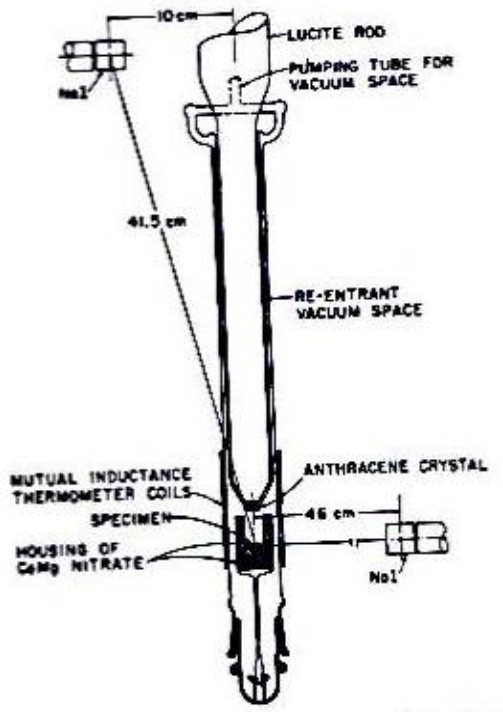
\includegraphics[width=0.6\linewidth]{parity_violation/wu_exp_opstelling.png}
    \caption{De experimentele opstelling van he Wu experiment}%
    \label{fig:parity_violation/wu_exp_opstelling}
\end{figure}

In figuur \ref{fig:parity_violation/wu_exp_opstelling} vindt je de opstelling van het Wu experiment. Hierbij is het zwarte blokje de bron waar CoMg nitraat in zit en dat gepolariseerd wordt met een magneet spoel. Er zijn 2 natrium jodide detectoren ($\gamma$ detectoren), 1 geplaatst rechts van de bron ($90^\circ$) en 1 links bovenaan het experiment ($0^\circ$ of $180^\circ$). Het verschil tussen de 2 detectoren zal de polarisatie van nikkel geven. Er is een derde kleine detector juist boven de detector die het elektron meet en ziet of deze parallel of antiparallel wordt uitgestuurd.\\
Als we de polarisatie van de kern weten uit de $\gamma$ anisotropie dan gaan we op zoek naar een afhankelijkheid van het elektron met de hoek.
\begin{equation}
    \begin{aligned}
        \label{eq:wu_elektron}
        W_e \propto 1 + P\beta_e\cos\theta
    \end{aligned}
\end{equation}
Indien er een $\theta$ afhankelijkheid is en $\alpha \neq 0$ dan zal de pariteit niet behouden zijn. De resultaten van dit experiment kunnen gevonden worden in figuur \ref{fig:parity_violation/wu_resultaten}. In de eerste plot kan je voor (a) de counts vinden van de $\gamma$ detector onder $90^\circ$ en (b) de counts voor de $\gamma$ detector bij $0^\circ$. Als we het magneet veld uit zetten en Co laten opwarmen (de polarisatie laten werdwijnen) en de counts van de detectoren plotten in functie van de tijd kunnen we zien dat de polarisatie ook zal verdwijnen in de $\gamma$ detectoren en kunnen we de polarisatie van de kernen meten wat we in de tweede plot zien. Deze plots zullen hetzelfde blijven als het magneet veld wordt omgedraaid m.a.w. de pariteit is behouden voor EM. Dit zal niet zo zijn als we naar de polarisatie van de elektronen kijken. Als het magneet veld wordt omgedraaid krijgen we ook een omdraaiin van de elektron pariteit en is de pariteit dus niet behouden.

\begin{figure}[h]
    \centering
    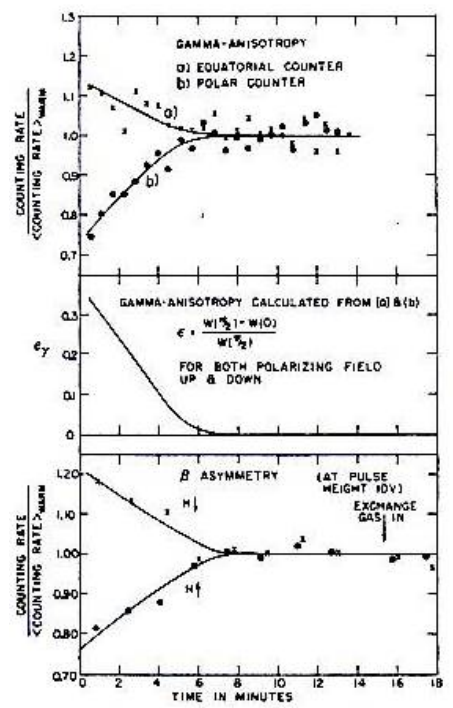
\includegraphics[width=0.6\linewidth]{parity_violation/wu_resultaten.png}
    \caption{Resultaten van het Wu experiment}%
    \label{fig:parity_violation/wu_resultaten}
\end{figure}

We kunnen schematisch zien wat er gebeurt met de spins van de deeltjes als het magneet veld wordt omgedraaid.

\begin{figure}[h]
    \centering
    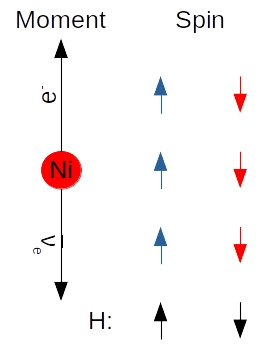
\includegraphics[width=0.4\linewidth]{parity_violation/wu.jpg}
    \caption{Schematische voorstelling van de spin in functie van het magnetisch veld}%
    \label{fig:parity_violation/wu}
\end{figure}

Hier wordt aangetoond dat $\alpha \approx 1$ is en de consistent is met een pariteit die maximaal geschonden zal worden. Uit de resultaten van dit experiment hebben Feynmann en Gell-Mann de V-A interactie opgesteld. In deze theorie is het elektron altijd links handig en het antineutrino rechts handig.
\begin{equation}
    \begin{aligned}
        \label{eq:v-a_theorie}
        \gamma^\mu \rightarrow \gamma^\mu (1-\gamma^5)
    \end{aligned}
\end{equation}
Er wordt naast de vector operator ook nog een axiale vector component toegevoegd $\gamma^\mu \gamma^5$. Om te zien hoe dit nu de pariteit juist schendt, kijken we terug naar de axiale stroom van de deeltjes.
\begin{equation}
    \begin{aligned}
        \label{eq:axiale_stroom_v-a}
        j^\mu &\propto \overline u(p')\gamma^\mu\gamma^5u(p)\\
        \gamma^5 &= i\gamma^0\gamma^1\gamma^2\gamma^3\\
                 &=
                 \begin{pmatrix}
                      0&0&1&0\\
                      0&0&0&1\\
                      1&0&0&0\\
                      0&1&0&0
                 \end{pmatrix}
    \end{aligned}
\end{equation}
Onder de pariteit operator verrandert deze axiale stroom als volgt:
\begin{equation}
    \begin{aligned}
        \label{eq:axiale_stroom_v-a_par}
        j^\mu = \overline u\gamma^\mu\gamma^5u \rightarrow \overline u\gamma^0\gamma^\mu\gamma^5\gamma^0u = -\overline u\gamma^0\gamma^\mu\gamma^0\gamma^5u
    \end{aligned}
\end{equation}
Het product van 2 van die axiale stromen zal nog steeds behouden zijn:
\begin{equation}
    \begin{aligned}
        \label{eq:axiale_stroom_v-a_prod}
        j_1\cdot j_2 = j_1^0j_2^0 - j_1^kj_2^k \rightarrow (-j_1^0)(-j_2^0) - j_1^kj_2^k = j_1\cdot j_2
    \end{aligned}
\end{equation}
Hetgene dat niet behouden is is de combinatie van de 2 stromen.
\begin{equation}
    \begin{aligned}
        \label{eq:stromen_v-a}
        j^\mu \propto \overline u (p') (g_V\gamma^\mu+g_A\gamma^\mu\gamma^5)u(p) &= g_Vj_V^\mu + g_Aj_A^\mu\\
        j_V^\mu &= \overline u(p')\gamma^\mu u(p)\\
        j_A^\mu &= \overline u(p')\gamma^\mu\gamma^5 u(p)
    \end{aligned}
\end{equation}
Het matrix element van deze gecombineerde stroom is
\begin{equation}
    \begin{aligned}
        \label{eq:v-a_matrix_el}
        \mathcal{M} \propto j_1\cdot j_2 = g_V^2j_1^V\cdot j_2^V + g_A^2j_1^A\cdot j_2^A + g_Vg_A(j_1^V\cdot j_2^A+j_1^A\cdot j_2^V)
    \end{aligned}
\end{equation}
De pariteit operator hierop uitwerkend geeft:
\begin{equation}
    \begin{aligned}
        \label{eq:v-a_stromen_par}
        j_1\cdot j_2 = g_V^2j_1^V\cdot j_2^V + g_A^2j_1^A\cdot j_2^A - g_Vg_A(j_1^V\cdot j_2^A+j_1^A\cdot j_2^V)
    \end{aligned}
\end{equation}
Hier is duidelijk te zien dat de pariteit niet is behouden voor de gemengde stroom. Deze schendende component is evenredig met $\propto \frac{g_Vg_A}{g_V^2+g_A^2}$ en is maximaal als $|g_V|=|g_A|$. De uiteindelijke V-A theorie geeft de volgende stroom:
\begin{equation}
    \begin{aligned}
        \label{eq:v-a_stromen_theorie}
        j^\mu \propto \overline u(p') \frac{1}{2} \gamma^\mu (1-\gamma^5)u(p)
    \end{aligned}
\end{equation}

\subsection{Heliciteit}%
\label{sub:heliciteit}

Keren we terug naar de handigheid wat hier belangrijk zal zijn.
\begin{equation}
    \begin{aligned}
        \label{eq:handigheid}
        h = \frac{\vec{S} \cdot \vec{p}}{|\vec{p}|} 
    \end{aligned}
\end{equation}
Dit is niets meer dan de spin geprojecteerd op de bewegingsrichting. De eigenwaardes van de heliciteit voor spin 1/2 deeltjes zijn $\pm \frac{1}{2}$. De heliciteit zal commuteren met de dirac hamiltoniaan, $[\hat{H}_D, \hat{h}]=0$. Belangrijk is wel dat de heliciteit niet Lorentz invariant is.

\subsection{Chiraliteit}%
\label{sub:chiraliteit}

Een grootheid dat nauw verwant is met de helicteit is de chiraliteit. Die gegeven worden door de volgende projectie operatoren:
\begin{equation}
    \begin{aligned}
        \label{eq:chiraliteit_operatoren}
        \begin{matrix}
            P_L = \frac{1-\gamma^5}{2} & P_R = \frac{1+\gamma^5}{2}
        \end{matrix}
    \end{aligned}
\end{equation}
Deze projecteren ofwel links- of rechtshandige deeltjes. Die zullen wel Lorentz invariant zijn. Omdat de $\gamma^5$ niet commuteert met de massa term van de hamiltoniaan zullen deze niet geconserveerd zijn voor massieve deeltjes. Wat deze nu juist uit projecteren is ofwel de linkshandige of rechtshandige component van een deeltje.
\begin{equation}
    \begin{aligned}
        \label{eq:proj_deeltjes}
        \begin{matrix}
            u_L = \frac{1}{2} (1-\gamma^5)u & u_R = \frac{1}{2} (1+\gamma^5)u\\
            \overline u_L = \overline u\frac{1}{2} (1-\gamma^5) & u_R = \overline u\frac{1}{2} (1+\gamma^5)
        \end{matrix}
    \end{aligned}
\end{equation}
Met deze info kan een relatie gevonden worden tussen de heliciteit en deze projectie operatoren.
\begin{equation}
    \begin{aligned}
        \label{eq:hel_chir}
        u_\uparrow &= \frac{1}{2} (1+\kappa)u_R + \frac{1}{2} (1-\kappa)u_L\\
        \kappa &= \frac{p}{E+m} 
    \end{aligned}
\end{equation}

\subsection{$f\overline f$-annihilatie}%
\label{sub:_foverline_f_annihilatie}

De annihilatie van een fermion-antifermion in een boson wordt gegeven door:
\begin{equation}
    \begin{aligned}
        \label{eq:fermion_annihilatie}
        \overline v \gamma^\mu \left( \frac{1-\gamma^5}{2} \right) u &= \overline v \gamma^\mu \left( \frac{1-\gamma^5}{2} \right)^2 u\\
                                                                     &= \overline v \left( \frac{1+\gamma^5}{2} \right) \gamma^\mu \left( \frac{1-\gamma^5}{2} \right) u\\
                                                                     &= \overline v_R \gamma^\mu u_L
    \end{aligned}
\end{equation}
Hier hebben we dus aangetoond dat we de V-A interactie kunnen zien als een vector interactie die bindt met linkschirale ($\approx$ linkshandig) deeltjes en rechtschirale ($\approx$ rechtshandige) antideeltjes. De heliciteit fractie is chirale toestanden kunnen gevonden worden door:

\begin{table}[h]
    \centering
    \label{tab:chir_hel}
    \begin{tabular}{c|cccc}
                        & $e^-/f$                   & $e^+/\overline f$         & $\nu$ & $\overline \nu$   \\
        \hline
        links handig    & $\frac{1}{2}(1+\kappa)$   & $\frac{1}{2}(1-\kappa)$   & $1$   & $0$               \\
        rechts handig   & $\frac{1}{2}(1-\kappa)$   & $\frac{1}{2}(1+\kappa)$   & $0$   & $1$               
    \end{tabular}
\end{table}
De polarisatie van $e^- = -\kappa \approx -\beta$. Het experiment om de polarisatie van het elektron te bepalen is interessant om te bekijken. De resultaten van deze experimenten wordt de polarisatie geplot in functie van $\beta$ wat evenredig moet zijn. 

\begin{figure}[h]
    \centering
    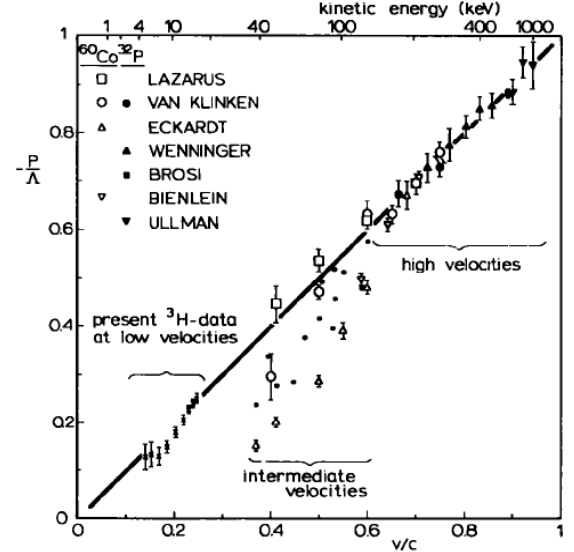
\includegraphics[width=0.5\linewidth]{parity_violation/pol_elektron.png}
    \caption{Resultaten van polarisatie experimenten van het elektron}%
    \label{fig:parity_violation/pol_elektron}
\end{figure}

Bij hoge energie werd deze relatie mooi gevolgd maar zagen dat dit niet het geval was bij lagere energieën. De vraag dat hier dus op komt is nu of de pariteit enkel wordt geschonden bij hoge energie en niet bij lage energie? Meneer Van Klinken onderzoekt nu deze polariasatie bij lage energie wat een heel leerrijk experiment was, zeker de manier waarop deze is opgesteld.

\begin{figure}[h]
    \centering
    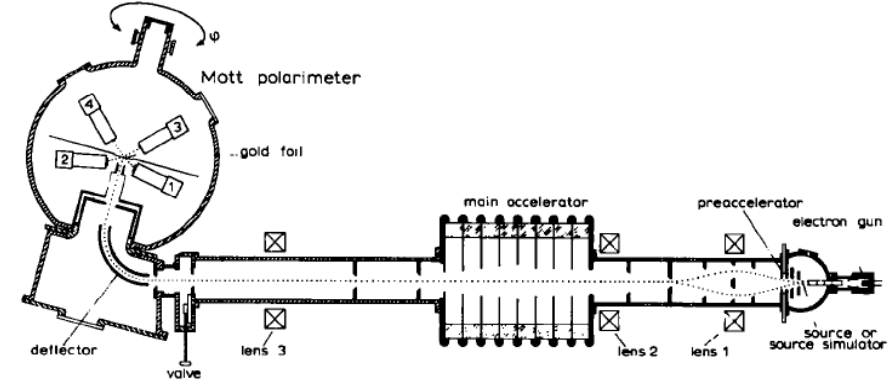
\includegraphics[width=0.8\linewidth]{parity_violation/van_klinken.png}
    \caption{Experimentele opstelling voor onderzoek naar elektron polarisatie bij lage energie}%
    \label{fig:parity_violation/van_klinken}
\end{figure}

Figuur \ref{fig:parity_violation/van_klinken} geeft een schematische voorstelling van het Van Klinken experiment. Hierbij worden elektronen aangemaakt in een elektronenbundel. Waar we enkel de elektronen behouden in een bepaalde chirale toestand. Vervolgens kunnen we deze elektronen versnellen (dit omdat de polarisatie dan makkelijker te bepalen is). De versnelde elektronen buigen we nu af naar de Mott polarimeter. De vraag is nu waarom we de elektronen afbuigen. Dit is door de manier waarop de polarimeter zal werken.\\
{\color{blue} Intermezzo: werking van de Mott polarimeter\\
    Deze zal gerbuik maken van de Mott scattering wat niets anders is dan een elastische $eN$-scattering. Het elektron wordt dus verstrooit in het Coulomb-veld en voelt een magnetisch veld $\propto -\vec{v}\times \vec{E}$. Dit komt overeen met het angulair moment. Het elektron zal van de kern deflecteren met $V \propto \vec{\mu} \cdot \vec{B}$. Het interessante is dat we de polarisatie van de spin enkel zullen kunnen waarnemen als de spin parallel staat op het magneetveld en dus loodrecht op zijn impuls staat.\\
    De Mott polarisatie is dus enkel gevoelig voor transversale polarisatie. Het is dus nodig om de spin of bewegingsrichting met $90^\circ$ te draaien.
}
Bij de afbuiging van deze elektronen moeten we dus enkel de bewegingsrichting aanpassen en niet de spin. We kunnen dus niet gebruik maken van magneten om deze afbuiging uit te voeren. In dit experiment maken we gebruik van een elektrostatische deflector die met elektrische velden werkt om de elektronen af te buigen en deze laat de spin gerust. Uit deze experimenten was het ook mogelijk om netjes te zien dat deze de relatie tussen polarisatie en $\beta$ volgen.

\subsection{Pion verval}%
\label{sub:pion_verval}

\begin{figure}[h]
    \centering
    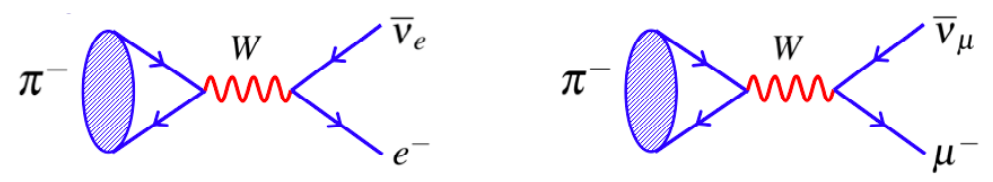
\includegraphics[width=0.8\linewidth]{parity_violation/pion_verval.png}
    \caption{Diagrammen van een pion verval}%
    \label{fig:parity_violation/pion_verval}
\end{figure}

Kijken we naar het verval van het pion naar ofwel het elektron of het muon met hun respectievelijke antineutrino zien we dat er geen verschil is tussen de 2 bij het annihileren van het $d\overline u$ paar naar het W boson. Het verschil zal hem ook niet zitten in de vertex waar het $W$ boson vervalt in de leptonen. In deze vertexen staan voor de elektromagnetische wisselwerking geen andere ladingen en dus elementen. Het verschil van deze diagrammen zal dus zitten in de faseruimte van deze processen. De faseruimte voor het verval naar elektronen zal veel groter zijn dan het verval naar muonen ($\Gamma_e \gg \Gamma_\mu$). Dit omdat het elektron veel minder weegt dan het muon en meer faseruimte over heeft. We verwachten dus dat het pion zo goed als altijd zou vervallen naar een elektron. Dit is niet wat we in de werkelijkheid zien waar zo goed als alle pionen vervallen in muonen. Dit vreemde gedrag kan makkelijk begrepen worden met behulp van de chiraliteits operator.\\
Gaan we uit van een stilstaant pion dat vervalt naar een muon en een een antineutrino. Hun impuls zal dus tegengesteld zijn.

\begin{figure}[h]
    \centering
    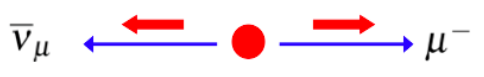
\includegraphics[width=0.8\linewidth]{parity_violation/pion_verval_kin.png}
    \caption{Schematische voorstelling van het pion verval naar muonen}%
    \label{fig:parity_violation/pion_verval_kin}
\end{figure}

Het antineutrino is massaloos en moet dus rechts handig zijn en is zijn spin dus gelijk aan zijn impuls richting. Omdat de totale spin van het pion 0 is moet de spin van het muon tegengesteld zijn en is dus ook rechtshandig. De zwakke interactie zal dit deeltje aanmaken met een linkse chiraliteit. De kan om een rechtshandig deeltje te bekomen kunnen we nu vinden door de eerder bepaalde relaties tussen chiraliteit en heliciteit, vergelijking (\ref{eq:hel_chir}). Het matrix element van dit verval wordt dus:
\begin{equation}
    \begin{aligned}
        \label{eq:pion_verval_matrix}
        \mathcal{M} \propto \left( 1 - \frac{p_l}{E_l + m_l} \right)
    \end{aligned}
\end{equation}
De breuk kunnen we aan de hand van 4 vector kinematica herschrijven. De 4 impulsen van deze deeltjes zijn:
\begin{equation}
    \begin{aligned}
        \label{eq:4_impuls_pion_verval}
        p_\pi &= (m_\pi,0,0,0)\\
        p_l &= (E_l, 0, 0, p_l)\\
        p_{\overline \nu} &= (p_l, 0, 0, -p_l)
    \end{aligned}
\end{equation}
Hierbij hebben we gebruik gemaakt dat het pion stil staat, dat het antineutrino stil staat en dat de impuls van het antineutrino en lepton tegengesteld zijn. Uit behoud van 4 impuls is het mogelijk om de $E_l$ te berekenen.
\begin{equation}
    \begin{aligned}
        \label{eq:berekenen_e_l}
        p_\pi &= p_l + p_{\overline \nu}\\
        p_\pi - p_l &= p_{\overline \nu}\\
        (p_\pi - p_l)^2 &= p_{\overline \nu}^2\\
        m_\pi^2+m_l^2-2m_\pi E_l &= 0\\
        E_l = \frac{m_\pi^2 + m_l^2}{2m_\pi}
    \end{aligned}
\end{equation}
Uit de massa energie relatie krijgen we $p_l$.
\begin{equation}
    \begin{aligned}
        \label{eq:berekenen_p_l}
        E_l^2 &= p_l^2 + m_l^2\\
        p_l^2 &= \left( \frac{m_\pi^2+m_l^2}{2m_l} \right)^2-m_l^2\\
        p_l = \frac{m_\pi^2-m_l^2}{2m_\pi} 
    \end{aligned}
\end{equation}
Dit kunnen we nu allemaal invullen in de originele breuk.
\begin{equation}
    \begin{aligned}
        \label{eq:omvormen_breuk_pion_verval}
        \frac{p_l}{E_l+m_l} &= \frac{\frac{m_\pi^2-m_l^2}{2m_\pi}}{\frac{m_\pi^2 + m_l^2}{2m_\pi}+m_l}\\
                            &= \frac{\frac{m_\pi^2-m_l^2}{2m_\pi}}{\frac{m_\pi^2 + m_l^2}{2m_\pi}+\frac{2m_\pi m_l}{2m_\pi}}\\
                            &= \frac{(m_\pi+m_l)(m_\pi-m_l)}{(m_\pi+m_l)^2}\\
                            &= \frac{((m_\pi-m_l)}{(m_\pi+m_l)}
    \end{aligned}
\end{equation}
Zo kunnen we inzien dat het matrix element proportioneel wordt als volgt:
\begin{equation}
    \begin{aligned}
        \label{eq:pion_verval_matrix_2}
        \mathcal{M} \propto \frac{m_l}{m_\pi + m_l} 
    \end{aligned}
\end{equation}
Voor de stromen van dit verval hebben we voor de leptonische stroom
\begin{equation}
    \begin{aligned}
        \label{eq:pion_verval_lept_stroom}
        j_l^\nu = \frac{g_W}{\sqrt{2}} \overline u(p_l) \frac{1}{2} \gamma^\nu (1-\gamma^5)v(p_{\overline \nu})
    \end{aligned}
\end{equation}
en de pion stroom voor een gebonden hadron is er maar 1 relevante 4 vector $p_\pi$
\begin{equation}
    \begin{aligned}
        \label{eq:pion_verval_pion_stroom}
        j_\pi^\mu = \frac{g_W}{\sqrt{2}} \frac{1}{2} f_\pi p_\pi^\mu
    \end{aligned}
\end{equation}
Ten laatste zal er ook nog een propagator term zijn $ \frac{g_{\mu\nu}}{m_W^2} $. Het matrix element wordt nu
\begin{equation}
    \begin{aligned}
        \label{eq:pion_verval_matrix_3}
        \mathcal{M}_{fi} &= \frac{g_W}{\sqrt{2}} \frac{1}{2} f_\pi p_\pi^\mu \frac{g_{\mu\nu}}{m_W^2} \frac{g_W}{\sqrt{2}} \overline u(p_l) \frac{1}{2} \gamma^\nu (1-\gamma^5)v(p_{\overline \nu})\\
                         &= \frac{g_W^2}{4m_W^2} g_{\mu\nu} f_\pi p_\pi^\mu \overline u(p_l) \gamma^\nu \frac{1}{2} (1-\gamma^5)v(p_{\overline \nu})\\
                         &= \frac{g_W^2}{4m_W^2} f_\pi m_\pi \overline u(p_l) \gamma^0 \frac{1}{2} (1-\gamma^5)v(p_{\overline \nu})\\
                         &= \frac{g_W^2}{4m_W^2} f_\pi m_\pi \overline u^\dagger(p_l) \frac{1}{2} (1-\gamma^5)v(p_{\overline \nu})\\
                         &= \frac{g_W^2}{4m_W^2} f_\pi m_\pi \overline u^\dagger(p_l)v_\uparrow(p_{\overline \nu})
    \end{aligned}
\end{equation}
Het belangrijke dat hier onthouden moet worden is dat voor de leptonen het matrix element mooi kan uitgeschreven worden maar dat dit niet lukt voor het pion. De "blob" van het pion wordt samengebracht in een factor $f_\pi$. Uiteindelijk bekomen we een links chiraal deeltje dat bindt met een rechtshandig antideeltje door de zwakke wisselwerking. Om de waarschijnlijkheid hiervan te bekijken moeten we kijken wat de fractie aan rechtse heliciteit is van het links chirale deeltje door het behoud van angulair moment. Zoals we eerder hebben uitgerekend zien we dan dat het matrix element herschreven kan worden tot
\begin{equation}
    \begin{aligned}
        \label{eq:pion_verval_matrix_final}
        \mathcal{M}_{fi} &= \frac{g_W^2}{4m_W^2} f_\pi m_\pi \sqrt{E_l+m_l}\sqrt{p}\left( 1 - \frac{p}{E_l+m_l} \right)\\
                         &= \left( \frac{g_W^2}{4m_W^2} \right)^2 f_\pi m_l \sqrt{m_\pi^2-m_l^2}
    \end{aligned}
\end{equation}
Het uiteindelijke matrix element moet gekwadrateerd worden en krijgen we 
\begin{equation}
    \begin{aligned}
        \label{eq:pion_verval_matrix_final_kwad}
        \left<|\mathcal{M}_{fi}|^2\right> = |\mathcal{M}|^2 &= 2G_F^2 f_\pi^2m_l^2(m_\pi^2-m_l^2)\\
        \frac{G_F}{\sqrt{2}} &= \frac{g_W^2}{8m_W^2}
    \end{aligned}
\end{equation}
Hier niet zo belangrijk maar we hebben de Lorentz invariante faseruimte nog nodig $ \frac{4\pi}{32\pi^2m_\pi^2} p$. Samen met het matrix element geeft dit de verval breedte
\begin{equation}
    \begin{aligned}
        \label{eq:pion_verval_breedte}
        \Gamma = \frac{4\pi}{32\pi^2m_\pi^2} p \left<|\mathcal{M}_{fi}|^2\right> = \frac{G_F^2}{8\pi m_\pi^3} f_\pi^2 \left( m_l(m_\pi^2-m_l^2) \right)^2
    \end{aligned}
\end{equation}
Het belangrijke dat we moeten inzien is dat de ratio tussen de 2 verval modes van het pion afhangen van de massa's van de deeltjes.
\begin{equation}
    \begin{aligned}
        \label{eq:pion_verval_ratio}
        \frac{\Gamma(\pi^- \rightarrow e^-\overline \nu_e)}{\Gamma(\pi^- \rightarrow \mu^-\overline \nu_\mu)}  = \left( \frac{m_e(m\pi^2 - m_e^2)}{m_\mu(m\pi^2 - m_\mu^2)} \right) = 1.26 \times 10^{-4}
    \end{aligned}
\end{equation}

\end{document}
